\documentclass[a4paper,12pt]{article}
\usepackage{amsmath}
\usepackage{graphicx}
\usepackage{hyperref}
\usepackage[utf8]{inputenc}
\usepackage[english,bulgarian]{babel}
\usepackage{amsthm}
\usepackage{mathtools}
\usepackage{graphicx}
\usepackage{amsfonts}
\usepackage{amssymb}

\title{Решения на задачите по ОТО}
\author{Ирина Валентинова Христова, 82071}
\begin{document}
\maketitle
\pagebreak
\section*{Задача 1.}
Спрямо СТО времето в различните инерциални отправни системи, движещи се с 
различни скорости спрямо една абсолютна (или "лабораторна") инерциална отправна система,
тече по различен начин.

Оттук възниква и т. нар. "парадокс на близнаците". Нека приемем, че имаме двама близнаци, 
единият от които е в покой спрямо инерциалната (приемаме я за такава) отправна система, свързана
със Земята, а другият близнак е в покой спрямо интерциалната отправна система, свързана 
с космичеки кораб, който се движи с постоянна скорост спрямо Земята.

Нека разгледаме близнака, намиращ се на Земята. От негова гледна точка,
космическият кораб се отдалечава с постоянна скорост и спрямо СТО времето в отправната система, 
свързана с кораба, тече по-бавно. Това означава, че след като пътуващият на космическия кораб близнак се завърне на Земята, 
той трябва е по-млад от близнака, който през цялото време е бил на Земята.

Нека разгледаме близнака, движещ се на космическия кораб. От негова гледна точка Земята се отдалечава от него с постоянна 
скорост, т.е. времето тече по-бавно за близнака, който се намира на Земята. Това означава, че след като двамата близнаци се срещнат отново, 
от гледна точка на близнака в космическия кораб, другият близнак ще бъде по-млад от него.

Така стигаме до извода, че спрямо който и да е от двамата близнаци, другият ще е по-млад след като се срещнат, което не е възможно.

До това противоречие стигнахме след предположението, че двете отправни системи са напълно равноправни, 
защото СТО ни казва, че физическите явления във всеки две инерциални отправни системи са напълно еднакви.

Решението на този "парадокс" лежи в това, че за да се върне космическият кораб на Земята, трябва да промени посоката на скоростта си. 
Тази промяна на посоката на скоростта неизбежно е свързана с появата на ускорение, защото дори и корабът да се движи с постоянна по големина скорост през цялото време, 
неизбежно ще възникне поне центростремително ускорение. Това означава, че близнакът, който е на космическия кораб, ще може да разбере с физически експеримент на кораба, че изпитва ускорение
и неговата отправна система не е инерциална. Така възниква неравнопоставеност между 
двете отправни системи и наистина двамата близнаци ще са на различни години след като се срещнат (близнакът на Земята ще бъде по-стар).

Това се потвърждава и от математическия апарат на СТО.
\pagebreak
\section*{Задача 2.}
От уравненията на Максуел следва, че скоростта на електромагнитните 
вълни във вакуум има определена скорост
$c \approx 3.10^{8} m/s$.

Трябва да знаем в коя отправна система се измерва тази скорост, 
защото съгласно Галилеевия закон за събиране на скорости,
скоростта на светлината би трябвало да е различна в различните отправни системи.

Нека си представим една хипотетична среда, която изпълва цялото пространство и минава през всички тела. 
По времето на Майкелсон учените са предполагали, че такава среда съществува и електромагнитните вълни 
представляват трептения на тази среда. Наричали са я ефир. Предполагало се е, че уравненията на Максуел имат 
своя обичаен вид само в отправна система, свързана с ефира.
Това означава, че в електродинамиката би трябвало да съществува привилегирована
инерциална отправна система, в която ефирът е неподвижен. 
По този начин уравненията на Максуел имат различен вид във всички други отправни системи
и следователно скоростта на електромагнитните вълни (в частност на светлината)
е различна в тези отправни системи.

По това време една от основните задачи на физиците е била откриването на т. нар. 
ефирен вятър, който представлява движението на ефира в различните отправни системи.
Един от основните експерименти с тази цел е опитът на Майкелсон и Морли.
Те искат да измерят скоростта на абсолютно движение на Земята спрямо тази привилегирована отправна система, свързана 
с ефира. 
Така те конструират интерферометърът на Майкелсон.
\begin{center}
    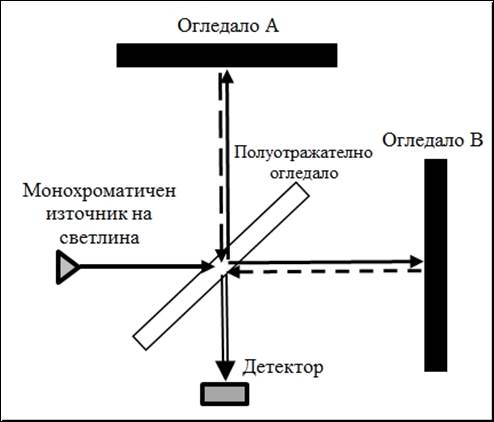
\includegraphics{image01.jpg}
\end{center}

Сноп монохроматична светлина преминава през полуотражателно огледало, 
върху едната повърхност на което е нанесен тънък слой метал. 
Светлината частично се отразява и частично преминава през него, 
и по този начин снопът светлина се разделя на 2 части, които се отразяват от огледало А и огледало B.
След това тези 2 части от снопа преминават отново през полуотражателното огледало и 
интерферират помежду си. Интерференчната картина може да се наблюдава в детектора. 

Нека двете рамена на интерферометъра имат еднаква дължина $l$. Това е разстоянието между 
полуотражателното огледало и двете огледала.
Ако скоростта на светлината е еднаква във всички направления, двата снопа ще изминат 
разстоянието $2l$ от полуотражателното огледало до двете огледала и обратно за еднакво време $t=\frac{2l}{c}$
и не би възникнала фазова разлика между двете вълни.
Нека приемем, че Земята се движи заедно с интерферометъра със скорост $v$ спрямо ефира.
За наблюдател от Земята ефирът се движи в противоположна посока със скорост $v$.
Според теорията на ефира скоростта на светлината е $c$ спрямо неподвижния ефир.
Галилеевият закон за събиране на скорости ни казва, че снопът до огледало $B$ се 
движи със скорост $c-v$ до огледалото, а скоростта на отразения сноп е $c+v$.
Този сноп ще измине разстоянието $2l$ за по-голямо време от снопа до огледало $A$.
Ако завъртим интерферометъра на $90^{\circ}$, тогава вторият сноп ще се движи в направление на 
ефирния вятър и ще закъснява. Следователно интерференчната картина трябва да се измести след завъртане на 
интерферометъра.
За получаването на добри резултати е трябвало измерванията да са с изключително добра точност
заради огромната разлика между скоростта на орбитално движение на Земята около Слънцето и скоростта на светлината.
Всички опити дават отрицателен резултат, т.е. че не е регистрирано отместване на интерференчната картина при завъртане 
на интерферометъра. Това показва, че ефирен вятър не съществува.
В съвременната наука се провеждат опити с лазери и гама лъчи, които показват с много голяма точност, че
скоростта на светлината във вакуум спрямо Земята е еднаква във всички направления.
\pagebreak
\section*{Задача 5.}
Метрика на Шварцшилд:
\begin{equation*}
    ds^2 = \left(1 - \frac{\alpha}{r}\right)c^2dt^2 - \frac{dr^2}{1 - \frac{\alpha}{r}} - r^2\left[ d\theta^2 + \sin^2\theta d\varphi^2 \right]
\end{equation*}
В координати $(ct, r, \theta, \varphi)$ само диагоналните
компоненти на метричния тензор са ненулеви: 
\begin{equation*}
\begin{pmatrix}
    1-\frac{\alpha}{r} & 0 & 0 & 0\\
    0 & -\frac{1}{1-\frac{\alpha}{r}} & 0 & 0 \\
    0 & 0 & -r^2 & 0 \\
    0 & 0 & 0 & -r^2\sin^2\theta
\end{pmatrix}
\end{equation*}

Ще пресметнем символите на Кристофел по формулата:
\begin{equation*}
    \varGamma^m_{ij} = \frac{1}{2}g^{mk}(g_{ki,j} + g_{kj,i}-g_{ij,k})
\end{equation*}

Тъй като недиагоналните членове са нула, т.е. $g^{mk}=0$ при $m \neq k$, следва:
\begin{equation*}
    \varGamma^m_{ij} = \frac{1}{2}g^{mm}(g_{mi,j}+g_{mj,i} - g_{ij, m})
\end{equation*}

Тъй като компонентите на метричния тензор не зависят от $t$ или $\varphi$, то:

    $g_{ij, 0} = \frac{\partial g_{ij}}{\partial t} =0$ и 
    $g_{ij, 3} = \frac{\partial g_{ij}}{\partial \varphi} =0$ \\

    Пресмятаме: 

    \begin{equation}
        \begin{aligned}
        \varGamma^0_{01} = \frac{1}{2}g^{00}\left(\frac{\partial g_{00}}{\partial r} + \frac{\partial g_{01}}{\partial t} - \frac{\partial g_{01}}{\partial t}\right) =\\
        = \frac{1}{2}\left( 1- \frac{\alpha}{r}\right)^{-1} \frac{\partial}{\partial r}\left(1 - \frac{\alpha}{r}\right) =\\
        = \frac{1}{2}.\frac{1}{1 - \frac{\alpha}{r}}.\frac{\alpha}{r^2} = \frac{\alpha}{2r^2}.\frac{1}{\frac{r-\alpha}{r}} =\\ 
        = \frac{\alpha}{2r(r-\alpha)}
        \end{aligned}
    \end{equation}
    \newline

    \begin{equation}
        \begin{aligned}
        \varGamma^1_{11} = \frac{1}{2}g^{11}\left(\frac{\partial g_{11}}{\partial r} + \frac{\partial g_{11}}{\partial r} - \frac{\partial g_{11}}{\partial r}\right) =\\
        = \frac{1}{2}\left[ - \left( 1- \frac{\alpha}{r}\right)\right] \frac{\partial}{\partial r}\left(- \frac{1}{1-\frac{\alpha}{r}}\right) =\\
        = \frac{1}{2}.\left( 1- \frac{\alpha}{r}\right).\frac{r -\alpha - r}{(r-\alpha)^2} =\\ 
        = \frac{1}{2}.\frac{r-\alpha}{r}.\frac{(-\alpha)}{(r-\alpha)^2} = \\
        = -\frac{\alpha}{2r(r-\alpha)}
        \end{aligned}
    \end{equation}
    \newline

    \begin{equation}
        \begin{aligned}
        \varGamma^1_{00} = \frac{1}{2}g^{11}\left(\frac{\partial g_{10}}{\partial t} + \frac{\partial g_{10}}{\partial t} - \frac{\partial g_{00}}{\partial r}\right) =\\
        = -\frac{1}{2}\left( 1- \frac{\alpha}{r}\right).(-1).\frac{\partial}{\partial r}.\left( 1- \frac{\alpha}{r}\right) =\\
        = \frac{1}{2}.\left( 1- \frac{\alpha}{r}\right).\frac{\alpha}{r^2} =\\ 
        = \frac{1}{2}.\frac{r-\alpha}{r}.\frac{(-\alpha)}{(r-\alpha)^2} = \\
        = -\frac{\alpha(r-\alpha)}{2r^3}
        \end{aligned}
    \end{equation}
    \newline

    \begin{equation}
        \begin{aligned}
        \varGamma^2_{21} = \frac{1}{2}g^{22}\left(\frac{\partial g_{22}}{\partial t} + \frac{\partial g_{21}}{\partial \theta} - \frac{\partial g_{21}}{\partial \theta}\right) =\\
        = \frac{1}{2}\left(- \frac{1}{r^2}\right).\left[\frac{\partial}{\partial r}.(-r^2)\right] = - \frac{1}{2r^2}(-2r) = \frac{1}{r}
        \end{aligned}
    \end{equation}
    \newline

    \begin{equation}
        \begin{aligned}
        \varGamma^3_{31} = \frac{1}{2}g^{33}\left(\frac{\partial g_{33}}{\partial r} + \frac{\partial g_{31}}{\partial \varphi} - \frac{\partial g_{31}}{\partial \varphi}\right) =\\
        = -\frac{1}{2}\frac{1}{r^2\sin^2\theta}.\frac{\partial}{\partial r}(-r^2\sin^2\theta) = \\
        = \frac{1}{2} \frac{1}{r^2\sin^2\theta}.2r\sin^2\theta = \frac{1}{r}
        \end{aligned}
    \end{equation}
    \newline

    \begin{equation}
        \begin{aligned}
        \varGamma^1_{22} = \frac{1}{2}g^{11}\left(\frac{\partial g_{12}}{\partial \theta} + \frac{\partial g_{12}}{\partial \theta} - \frac{\partial g_{22}}{\partial r}\right) =\\
        = -\frac{1}{2}\left(1- \frac{\alpha}{r}\right).(-1).\frac{\partial}{\partial r}.(-r^2) = \\
        = -\frac{1}{2} \left(1-\frac{\alpha}{r}\right).2r = \\
        = - \frac{r-\alpha}{r}.r = \alpha - r
        \end{aligned}
    \end{equation}
    \newline

    \begin{equation}
        \begin{aligned}
        \varGamma^1_{33} = \frac{1}{2}g^{11}\left(\frac{\partial g_{13}}{\partial \varphi} + \frac{\partial g_{13}}{\partial \varphi} - \frac{\partial g_{33}}{\partial r}\right) =\\
        = -\frac{1}{2}\left(1- \frac{\alpha}{r}\right).(-1).\frac{\partial}{\partial r}.(-r^2\sin^2\theta) = \\
        = -\frac{1}{2} \left(1-\frac{\alpha}{r}\right).2r\sin^2\theta = \\
        = - (\alpha - r)\sin^2\theta
        \end{aligned}
    \end{equation}
    \newline

    \begin{equation}
        \begin{aligned}
        \varGamma^2_{33} = \frac{1}{2}g^{22}\left(\frac{\partial g_{23}}{\partial \varphi} + \frac{\partial g_{23}}{\partial \varphi} - \frac{\partial g_{33}}{\partial \theta}\right) =\\
        = \frac{1}{2}\left(- \frac{1}{r^2}\right).(-1).\frac{\partial}{\partial \theta}.(-r^2\sin^2\theta) = \\
        = -\frac{1}{2r^2}.2r^2\sin\theta\cos\theta = \\
        = -\sin\theta\cos\theta
        \end{aligned}
    \end{equation}
    \newline

    \begin{equation}
        \begin{aligned}
        \varGamma^3_{32} = \frac{1}{2}g^{33}\left(\frac{\partial g_{33}}{\partial \theta} + \frac{\partial g_{32}}{\partial \varphi} - \frac{\partial g_{32}}{\partial \varphi}\right) =\\
        = -\frac{1}{2}\frac{1}{r^2\sin^2\theta}.\frac{\partial}{\partial \theta}.(-r^2\sin^2\theta) = \\
        = \frac{1}{2r^2\sin^2\theta}.r^2\sin\theta\cos\theta = \\
        = \cot\theta
        \end{aligned}
    \end{equation}
    \newline
    Окончателно получаваме за ненулевите символи на Кристофел:


    \begin{equation*}
        \begin{aligned}
        \varGamma^0_{01} = - \varGamma^1_{11} = \frac{\alpha}{2r(r-\alpha)} \\ 
        \varGamma^1_{00} = \frac{\alpha(r-\alpha)}{2r^3} \\ 
        \varGamma^1_{22} = \alpha - r \\
        \varGamma^2_{21} = \varGamma^3_{31} = \frac{1}{r} \\
        \varGamma^1_{33} = (\alpha - r)\sin^2\theta \\
        \varGamma^2_{33} = - \sin\theta\cos\theta \\
        \varGamma^3_{32} = \cot\theta
    \end{aligned}
    \end{equation*}

    Тензор на Ричи:
    \begin{equation*}
        R_{ik} = R^a_{iak} = \partial_k\varGamma^a_{ia} - \partial_a\varGamma^a_{ik}-\varGamma^a_{ba}\varGamma^b_{ik} + \varGamma^a_{bk}\varGamma^b_{ai}
    \end{equation*}

    Тъй като имаме пълна симетрия и ако си представим
    сферично-симетрична черна дупка в геометрия на Шварцшилд, ще имаме 
    цялата маса, съсредоточена в сингулярност, а извън нея всички компоненти на тензора на 
    Ричи ще бъдат нула.\\

    $R_{ik}=0 \forall i, k \in [0, 3]$\\

    Можем нагледно да го покажем за първата компонента:

    \begin{equation*}
        \begin{aligned}
            R_{00}=R^a_{0a0} = \partial_0\varGamma^a_{0a} - \partial_a\varGamma^a_{00}-\varGamma^a_{ba}\varGamma^b_{00}+\varGamma^a_{bo}\varGamma^b_{a0}=\\
            = - \partial_a\varGamma^a_{00} - \varGamma^a_{1a}\varGamma^1_{00}+\varGamma^0_{bo}\varGamma^b_{00} =\\
            = -\partial_a\varGamma^1_{00}-\varGamma^1_{11}\varGamma^1_{00}-\varGamma^2_{12}\varGamma^1_{00}-\varGamma^3_{13}\varGamma^1_{00}+\varGamma^0_{10}\varGamma^1_{00} = \\
            =- \frac{\partial}{\partial r}\left[ \frac{\alpha(r-\alpha)}{2r^3} \right] + \frac{\alpha}{2r(r-\alpha)}.\frac{\alpha(r-\alpha)}{2r^3}-2.\frac{1}{r}\frac{\alpha(r-\alpha)}{2r^3}
            + \frac{\alpha}{2r(r-\alpha)}.\frac{\alpha(r-\alpha)}{2r^3} = \\
            = -\alpha.\frac{2r^3 - 6r^3+6\alpha r^3}{4r^6} + \frac{\alpha^2}{2r^4} - \frac{\alpha(r-\alpha)}{r^4} = \\
            = \frac{4\alpha r^3 - 6 \alpha^2 r^2 + 2r^2\alpha^2-4r^3\alpha+4r^2\alpha^2}{4r^6} = 0
        \end{aligned}
    \end{equation*}

    Аналогично и за останалите компоненти $R_{ik}=0$.\\ \\
    Скаларната кривина е следната: $R=g^{ik}R_{ik}=0$.\\

    Тензорът на Риман: 
    \begin{equation*}
        R^i_{jkl}=\frac{\partial\varGamma^0_{10}}{\partial x^l} - \frac{\partial \varGamma^i_{jl}}{\partial x^k} + \varGamma^i_{al}\varGamma^a_{jk}-\varGamma^i_{ak}\varGamma^a_{jl}
    \end{equation*}

    Намираме ненулевите компоненти по следния начин: 
    \begin{equation*}
        \begin{aligned}
            R^0_{101} = \frac{\partial \varGamma^0_{10}}{\partial x^1} - \frac{\partial\varGamma^0_{11}}{\partial x^0}+ \varGamma^0_{a1}\varGamma^a_{10}
            - \varGamma^0_{a0}\varGamma^a_{11}= \\
            = \frac{\partial}{\partial r} \left( \frac{\alpha}{2r(r-\alpha)} \right)
            + \varGamma^0_{01}\varGamma^0_{10} - \varGamma^0_{10}\varGamma^1_{11} =\\
            = \frac{\alpha}{2}\frac{\partial}{\partial r}\left( \frac{1}{r^2-\alpha r} \right) + \left( \frac{\alpha}{2r(r-\alpha)} \right)^2 + \left( \frac{\alpha}{2r(r-\alpha)} \right)= \\
            = - \frac{(2r-\alpha)\alpha}{2(r^2-\alpha r)^2} + 2\frac{\alpha^2}{4r^2(r-\alpha)^2} = \\
            = \frac{\alpha(\alpha - 2r)}{2r^2(r-\alpha)^2} + \frac{2\alpha^2}{4r^2(r-\alpha)^2} = \frac{\alpha^2-2\alpha r + \alpha^2}{2r^2(r-\alpha)^2}= \\
            = \frac{2\alpha^2-2\alpha r}{2r^2(r-\alpha)} = -\frac{2\alpha(\alpha-r)}{2r^2(\alpha-r)^2} = - \frac{\alpha}{r^2(\alpha - r)}
        \end{aligned}
    \end{equation*}

    Оттук следва, че търсената компонента е:
    \begin{equation*}
        \begin{aligned}
            R_{0101} = g_{m0}R^0_{101} = g_{00}R^0_{101} = -\left( 1-\frac{\alpha}{r}\right).\frac{\alpha}{r^2(\alpha -r)} = - \frac{r-\alpha}{r}.\frac{\alpha}{r^2(\alpha-r)} = \frac{\alpha}{r^3}
        \end{aligned}
    \end{equation*}

    По аналогичен начин намираме:
    \begin{equation*}
        \begin{aligned}
            R^0_{202} = \frac{\partial\varGamma^0_{20}}{\partial x^2} - \frac{\partial\varGamma^0_{22}}{\partial x^0} + \varGamma^0_{a2}\varGamma^a_{20}-\varGamma^0_{a0}\varGamma^a_{22}
            = -\varGamma^0_{10}\varGamma^1_{22} = -\frac{\alpha}{2r(r-\alpha)}.(\alpha-r)=\frac{\alpha}{2r}
            \\
            R_{0202}=g_{00}R^0_{202} = \frac{\alpha}{2r}\left( 1-\frac{\alpha}{r} \right)
        \end{aligned}
    \end{equation*}
    \newline
    \begin{equation*}
        \begin{aligned}
            R^0_{303} = \frac{\partial \varGamma^0_{30}}{\partial x^3} - \frac{\partial\varGamma^0_{33}}{\partial x^0} + \varGamma^0_{a3}\varGamma^a_{30} - \varGamma^0_{a0}\varGamma^a_{33}
            = - \varGamma^0_ {10}\varGamma^1_{33} = -\frac{\alpha}{2r(r-\alpha)}.(\alpha-r)\sin^2\theta = \frac{\alpha\sin^2\theta}{2r}
            \\
            R_{0303}=g_{00}R^0_{303} = \left( 1- \frac{\alpha}{r} \right) \frac{\alpha\sin^2\theta}{2r} = \frac{\alpha(r-\alpha)\sin^2\theta}{2r^2}
        \end{aligned}
    \end{equation*}
    \newline
    \begin{equation*}
        \begin{aligned}
            R^1_{212} = \frac{\partial\varGamma^1_{21}}{\partial x^2} - \frac{\partial\varGamma^1_{22}}{\partial x^1} + \varGamma^1_{a2} + \varGamma^a_{21} - \varGamma^1_{a1}\varGamma^a_{22}
            = - \frac{\partial}{\partial r} (\alpha-r) + \varGamma^1_{12}\varGamma^1_{21}+\varGamma^1_{22}\varGamma^2_{21}-\varGamma^1_{11}\varGamma^1_{22} = \\
            =1 + (\alpha - r)\frac{1}{r}+\frac{\alpha}{2r(r-\alpha)}.(\alpha-r) = 1+\frac{\alpha-r}{r} - \frac{\alpha}{2r(r-\alpha)}(\alpha-r)=1+\frac{\alpha-r}{r}-\frac{\alpha}{2r} = \\
            = \frac{2r+2\alpha-2r-\alpha}{2r} = \frac{\alpha}{2r}
            \\
            R_{1212}=g_{11}R^1_{212}=-\frac{1}{1-\frac{\alpha}{r}}.\frac{\alpha}{2r}= - \frac{r}{r-\alpha}.\frac{\alpha}{2r}=-\frac{\alpha}{2(r-\alpha)} =\frac{\alpha}{2(\alpha-r)}
        \end{aligned}
    \end{equation*}
    \newline
    \begin{equation*}
        \begin{aligned}
            R^1_{313}=\frac{\partial\varGamma^1_{31}}{\partial x^3} - \frac{\partial\varGamma^1_{33}}{\partial x^1}+\varGamma^1_{a3}\varGamma^a_{31}-\varGamma^1_{a1}\varGamma^a_{33}
            = -\frac{\partial}{\partial r} [(\alpha-r)\sin^2\theta] + \varGamma^1_{33}\varGamma^3_{31} - \varGamma^1_{11}\varGamma^1_{33} = \\
            = \sin^2\theta + (\alpha-r)\sin^2\theta\frac{1}{r} + \frac{\alpha}{2r(r-\alpha)}(\alpha-r)\sin^2\theta
            = \sin^2\theta\left[ 1 + \frac{\alpha -r}{r} - \frac{\alpha}{2r} \right] = \sin^2\theta.\frac{\alpha}{2r}
            \\
            R_{1313}=g_{11}R^1_{313} = -\frac{1}{1-\frac{\alpha}{r}}.\frac{\alpha}{2r}.\sin^2\theta = \frac{\alpha\sin^2\theta}{2(\alpha-r)}
        \end{aligned}
    \end{equation*}
    \newline

    \begin{equation*}
        \begin{aligned}
            R^2_{323} = \frac{\partial\varGamma^2_{32}}{\partial x^3} - \frac{\partial\varGamma^2_{33}}{\partial x^2} + \varGamma^2_{a3}\varGamma^2_{32} - \varGamma^2_{a2}\varGamma^2_{33} = -\frac{\partial}{\partial\theta}(-\sin\theta\cos\theta) + \varGamma^2_{33}\varGamma^3_{32}-\varGamma^2_{22}\varGamma^2_{33}-\varGamma^2_{12}\varGamma^1_{33}= \\
            = \cos^2\theta-\sin^2\theta + (-\sin\theta\cos\theta)\cot\theta - \frac{1}{r}(\alpha-r)\sin^2\theta = -\sin^2\theta + \frac{r-\alpha-r}{r}=-\frac{\alpha}{r}\sin^2\theta
        \end{aligned}
    \end{equation*}

    \begin{equation*}
        R_{2323}=g_{22}R^2_{323}=-r^2.\left( -\frac{\alpha}{r} \right)\sin^2\theta=\alpha r\sin^2\theta
    \end{equation*}

    Окончателно: 
    \begin{equation*}
        R_{0101} = \frac{\alpha}{r^3} 
    \end{equation*}
    \begin{equation*}
        R_{0202} = \frac{\alpha(r-\alpha)}{2r^2} 
    \end{equation*}
    \begin{equation*}
        R_{0303} = \frac{\alpha(r-\alpha)\sin^2\theta}{2r^2} 
    \end{equation*}
    \begin{equation*}
        R_{1212} = \frac{\alpha}{2(\alpha-r)} 
    \end{equation*}
    \begin{equation*}
        R_{1313} = \frac{\alpha\sin^2\theta}{2(\alpha-r)} 
    \end{equation*}
    \begin{equation*}
        R_{2323} = \alpha r\sin^2\theta
    \end{equation*}

    \pagebreak
    \section*{Задача 6.}
    ФН: 82071 $\rightarrow$ Меркурий

    Точна формула за отместване на перихелия: \\
    Кеплеровото движение на една планета около Слънцето (т.е. в неговото гравитационно поле на Шварцшилд), може да се даде със следните 
    формули:

    $
        r(\varphi) = \frac{p}{1-e.\cos_q u}
    $
    или 
    $
        \frac{1}{r} = \frac{cn^2(\frac{u}{2})}{r_{min}} + \frac{sn^2(\frac{u}{2})}{r_{max}}
    $, 
    където $r(\varphi)$ е елиптична функция, а $r_{min}$ и $r_{max}$ са най-малкото и най-голямото
    разстояние от Слънцето до планетата. \\ \\
    Също така имаме, че: \\
    $
        r_{min} = (1-e)r_{\text{средно}}
    $ и 
    $
        r_{max}=(1+e)r_{\text{средно}}
    $, където $e$ е ексцентрицитетът на орбитата. \\
    \\ От полза ще ни бъде и следната формула: \\
    $p = \frac{2}{\frac{1}{r_{max}} + \frac{1}{r_{min}}}$. \\

    Можем да използваме следното диференциално уравнение: 
    \begin{equation*}
        \left( \frac{dr}{d\varphi} \right)^2 = \frac{c^2_1-h}{c^2_2}r^4 + \frac{ah}{c^2_2}r^3 - r^2+ar = \frac{dr(r-r_1)(r-r_{min})(r_{max}-r)}{r_1r_{min}r_{max}}
    \end{equation*}
    Oт формулите на Виет следва, че имаме следните равенства: \\
    $\frac{1}{\alpha} = \frac{1}{r_1} + \frac{1}{r_{min}} + \frac{1}{r_{max}}$ \\
    $\frac{1}{r_1} = \frac{1}{\alpha} - \frac{1}{r_{min}} - \frac{1}{r_{max}}$. \\
    \\
    Трябва да пресметнем елиптичните интеграли от първи род: 
    \begin{equation*}
        \begin{aligned}
            K = \int_{0}^{1} \frac{ds}{\sqrt[]{(1-s^2)(1-\kappa^2s^2)}}, \text{където } \kappa^2 = \frac{\frac{1}{r_{min}} - \frac{1}{r_{max}}}{\frac{1}{r_1} - \frac{1}{r_{max}}} \\
            K' = \int_{0}^{1} \frac{ds}{\sqrt[]{(1-s^2)(1-\kappa^{'2}s^2)}}, \text{където }\kappa^{'2} = 1-\kappa^2 \\
    \end{aligned}
    \end{equation*}

    Реалният период на $r$ по $\varphi$ е равен на:

    \begin{equation*}
        T = \frac{4K}{\sqrt[]{\frac{\alpha}{r_1} - \frac{\alpha}{r_{max}}}} = \frac{2\pi}{M\left(\sqrt[]{\frac{\alpha}{r_1} - \frac{\alpha}{r_{max}}}, \sqrt[]{\frac{\alpha}{r_1} - \frac{\alpha}{r_{min}}}\right)}
    \end{equation*} \\
    и следователно \\
    \begin{equation*}
        \varDelta\varphi = T- 2\pi = \frac{2\pi}{M\left(\sqrt[]{\frac{\alpha}{r_1} - \frac{\alpha}{r_{max}}}, \sqrt[]{\frac{\alpha}{r_1} - \frac{\alpha}{r_{min}}}\right)} - 2\pi
    \end{equation*}

    За Слънцето гравитационният радиус може да се намери по следния начин:
    \begin{equation*}
        \alpha = 2\frac{GM}{c^2} \approx 2. \frac{6,679.10^{-11}m^3kg^{-1}s^{-2} . 1,989.10^{30}kg}{(299 792 458m/s)^2} \approx 2, 95km
    \end{equation*}
Намираме: \\
    \begin{equation*}
        \begin{aligned}
            1 - \frac{\alpha}{r_{min}} - \frac{2\alpha}{r_{max}} \approx 0, 99999985 \\
            1 - \frac{2\alpha}{r_{min}} - \frac{\alpha}{r_{max}} \approx 0,99999983 \\
            \implies \varDelta\varphi \approx 2\pi \left( \frac{1}{0,99999984} - 1 \right) \approx 1, 005.10^{-6}
        \end{aligned}
    \end{equation*}

    Отместването по перихелия по точната формула е: \\ 
    $\approx \varDelta\varphi * \frac{100\text{ години}}{87, 969 \text{ дни}} \approx 41''$ \\

    Приближение на Айнщайн:
    \begin{equation*}
        \begin{aligned}
            \varDelta\varphi \frac{2\pi}{M\left( 1-\frac{\alpha}{2r_{min}} - \frac{\alpha}{r_{max}}, 1-\frac{\alpha}{r_{min}} - \frac{\alpha}{2r_{max}} \right)} - 2\pi \approx 
            \frac{2\pi}{1 - \frac{3\alpha}{\varphi r_{min}} - \frac{3\alpha}{4r_{max}}} - 2\pi \approx \\
            \approx \frac{3}{2}.\frac{\pi\alpha}{\frac{1}{r_{min}} + \frac{1}{r_{max}}} = \frac{3}{2}\pi\alpha \frac{1+e+1-e}{r_{\text{средно}(1-e)(1+e)}} = \frac{3\pi\alpha}{r_{\text{средно}(1-e^2)}} \rightarrow \text{формула на Айнщайн}
        \end{aligned}
    \end{equation*}

    \begin{equation*}
        \varDelta\varphi \approx \frac{3\pi\alpha}{r_{text{средно}}(1-e^2)} \approx 43''
    \end{equation*}

    Получихме резултати за отместването на перихелия на Меркурий по точната формула и по тази на Айнщайн.
\end{document}